\documentclass[12pt,a4paper]{article}
\usepackage{fancyhdr}\usepackage{graphicx}\usepackage{placeins}\usepackage{adjustbox}
\begin{document}
\pagestyle{fancy}\fancyhf{}\chead{Short summary report}
\begin{table}[t]\centering\caption {rnaQUAST metrics for assembled transcripts. In each row the best values are indicated with \textbf{bold}. For the transcript metrics (rows 2, 3) we highlighted the best \textbf{relative} values i.e. divided by the total number of transcripts in the corresponding assembly.}\begin{adjustbox}{width=1\textwidth}\small\begin{tabular}{|l*{7}{|r}|}\hline\textbf{METRICS/TRANSCRIPTS}                            & \textbf{Pdum\_new\_ref.Trinity.renamed.long} & \textbf{Pdum\_new\_ref.rnaSPAdes.renamed.long} & \textbf{Pdum\_new\_ref\_rnabloom.transcripts.renamed} & \textbf{Pele\_new\_ref.Trinity.renamed.long} & \textbf{Pele\_new\_ref.rnaSPdes.renamed.long} & \textbf{Pele\_new\_ref\_rnabloom.transcripts.renamed} \\ \hline\hline
\multicolumn{7}{l}{\bf BASIC TRANSCRIPTS METRICS}                                         \\ \hline
Transcripts                                             & 665918                           & 287218                             & 706997                                   & 1152755                          & 433491                            & 1274064                                  \\
Transcripts $>$ 500 bp                                  & 393538                           & 171434                             & 573533                                   & 587876                           & 200458                            & \textbf{807602}                          \\
Transcripts $>$ 1000 bp                                 & 247058                           & 120548                             & 483707                                   & 321193                           & 121478                            & \textbf{585204}                          \\ \hline
\end{tabular}\end{adjustbox}\end{table}
\FloatBarrier\clearpage\lfoot{generated by rnaQUAST}
\begin{figure}[t]\centering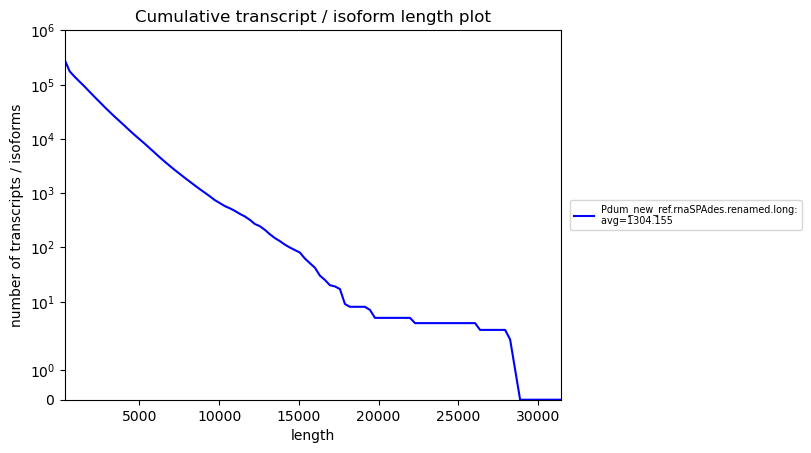
\includegraphics[width = \linewidth]{/mnt/c/worms/transcriptomes/rna_quast_results/comparison_output/transcript_length.png}\caption{Plot showing cumulative transcript length distribution. Each point represents the number of transcripts in the assembly with the corresponding length or longer; black dashed line corresponds to the database isoforms; the plot is given in logarithmic scale.}\end{figure}\FloatBarrier\clearpage
\end{document}